\subsection{GenII und GenIII Honeynets}
GenII Honeynets wurden entwickelt, um die Probleme der ersten Version zu beheben. Dabei soll das System allgemein leichter aufzustellen, und schwieriger zu entdecken sein. Die meisten Änderungen wurden bei der Datenkontrolle unternommen. Die Architektur eines Honeynets der zweiten Generation unterscheidet sich signifikant zu der eines GenI Honeynets. In Abb. \ref{hnet:genii} befindet sich eine Beispielarchitektur eines GenII Honeynets\cite{spitzner.2002a}\cite{WebGenII.2006b}.\\

\begin{figure}[h]
    \centering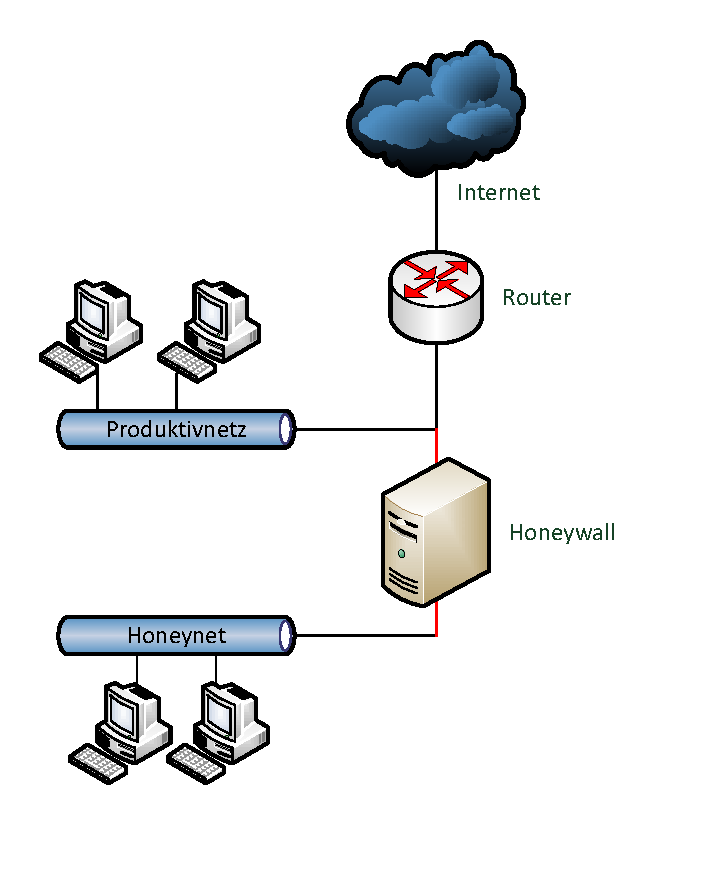
\includegraphics[scale=0.5]{Bilder/GenII.pdf}
  \caption{GenII Honeynet}
  \label{hnet:genii}
\end{figure}

\newpage
\noindent\textbf{Methoden zur Datenkontrolle}\\
\noindent GenI Honeynets erhalten ihre Datenkontrolle durch eine Limitierung der ausgehenden Verbindungen über eine Layer 3 Firewall. Das Problem hierbei war die relativ einfache Möglichkeit für den Angreifer herauszufinden, das es sich um ein Honeynet handelt (durch testen der Anzahl von ausstehenden Verbindungen oder TTL-Zähler). Die Layer 3 Firewall und das IDS werden in einem GenII Honeynet in einem Gerät, der Honeywall oder dem Honeynet Sensor, kombiniert\cite{WebGenII.2006b}. Dieser Sensor ist ein Layer 2 Gerät, ähnlich einer Bridge, welches es erschwert das Gerät ausfindig zu machen (TTL-Zähler wird nicht mehr dekrementiert, Pakete werden nicht geroutet). Jedoch wird jedes Paket welches das Honeynet empfängt oder verlässt den Sensor passieren\cite{spitzner.2002a}.
Durch die Verwendung eines Layer 2 Gerätes, befindet sich das Honeynet nicht mehr in einem separaten Netzwerk. In Abb. \ref{hnet:genii} trennt der Honeynet Sensor das Honeynet vom Produktivnetzwerk, in Wirklichkeit handelt es sich um das selbe Netz. Die Separierung der Netze findet nun auf Layer 2 statt auf Layer 3 statt.
Eine Weitere Änderung besteht in der Benutzung des IDS als Gateway. Dabei übernimmt das IDS die Funktion einer "intelligenten" Firewall, die erkennt, ob eine Verbindung legitim ist, oder ob es sich dabei um einen Angriff handelt. Zudem kann sie wie eine Firewall Verbindungen blockieren oder limitieren. Das IDS Gateway besitzt eine Signaturdatenbank, in der bekannte Angriffsmuster enthalten sind. Wir ein solches Muster erkannt, kann das IDS die Verbindung blockieren\cite{spitzner.2002a}. 
Ein Vorteil dieser Methode ist, das der Angriff nicht mehr über die ausgehenden Verbindungen identifiziert werden muss, sondern schon im voraus klar ist, was der Hacker plant. So kann verhindert werden, das der Angreifer mit seinen limitierten ausgehenden Verbindungen Schaden anrichtet. Angriffsmuster, die nicht in der Datenbank des IDS verzeichnet sind, werden als legitime Aktion angesehen. Deswegen werden meist die ausgehenden Verbindungen über das IDS weiterhin, wie in GenI, limitiert. Jedoch können hier weitaus größere Werte in Betracht gezogen werden, so dass das Fingerprinting ebenfalls erschwert wird\cite{spitzner.2002a}.
Ein anderen Vorteil dieser Vorgehensweise besteht darin, dass das GenII Honeynet auf unautorisierte Aktionen antworten kann. Versucht der HAcker von einem kompromittierten Honeypot einen Produktiv-Rechner anzugreifen, so wird das Paket vom IDS abgefangen, modifizieren um den Angriff zu neutralisieren, und eine unverständliche Antwort an den Hacker zurückschicken. Der Angreifer sieht zwar, dass sein Angriff gestartet wurde, sein Exploit ist aber nie erfolgreich.
Ein Beispiel für ein solches IDS-Gateway ist Hogwash\cite{spitzner.2002a}.\\

\noindent\textbf{Methoden zur Datenaufzeichnung}\\
\noindent Die Möglichkeiten zu Datenaufzeichnung der zweiten Generation unterscheiden sich kaum zu denen der Ersten. Die meisten Informationen werden durch das IDS gesammelt. Dateien die lokal auf den Honeypots aufgezeichnet werden, werden weiterhin auf einem Log-Server zusätzlich gespeichert. Die Probleme der ersten Generation bleiben hier vorerst weiterhin bestehen. Bei verschlüsselten Kommunikationen und Ausschalten der syslog-Funktion, bleiben nur die Daten, die über das IDS gesammelt werden können. Diese Probleme werden in der dritten Generation behoben\cite{spitzner.2002a}.\\
\newpage

\noindent\textbf{Methoden zur Datensammlung}\\
\noindent Die Datensammlung spielt eine Rolle, wenn mehrere Honeynets Daten zu einer zentralen Datensammelstelle senden. Für einfache Honeynets findet die Datensammlung auf einem Log-Server innerhalb des Honeynets statt. Für verteilte Honeynets muss ein zentraler Log Server für alle Honeynets bereitstehen. Wichtig für diesen ist, dass die Daten sicher und unverändert vom Honeynet auf das System gelangen (z.B. über einen IPSec Tunnel vom Honeynet zum zentralen Log-Server). 
Ein anderer Aspekt der beachtet werden muss ist der, dass die Daten die gesammelt werden standardisiert werden müssen. Daten die von verschiedenen Honeynets stammen sollten alle das gleiche Format haben und eindeutig einem Honeynet zuweisbar sein\cite{spitzner.2002a}. \\

\noindent\textbf{GenIII Honeynets und Zukunft}\\
\noindent Ende 2004 wurde die vorerst letzte Generation von Honeynets vorgestellt. Ein GenIII Honeynet besitzt die selbe Netzwerkarchitektur wie dessen Vorgänger, behebt jedoch einig dessen Schwachstellen. Bei dem Versuch einen Honeynet Standard zu schaffen, und eine Möglichkeit zu finden, ein Honeynet leichter zu erstellen, hat das Honeynet-Project eine CD entwickelt, die alle Anforderungen eines Honeynets beinhaltet. Diese CD (\emph{Roo} genannt) wird als dritte Generation angesehen. Die aktuelle Version (1.4, Stand: 2014) bietet neben der verbesserten Datenaufzeichnung, eine grafische Web-Oberfläche zur Datenanalyse, und unterstützt weiter Tools wie Sebek und Hflow2 (Siehe Kapitel Tools)\cite{WebGenIII.2006b}.